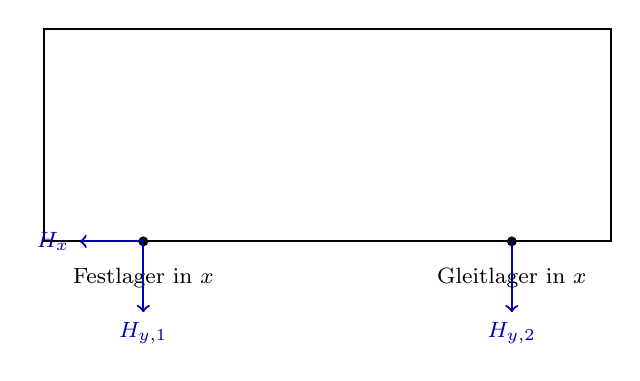
\begin{tikzpicture}[scale=0.9, every node/.style={font=\footnotesize}]
\draw[thick] (0,0) rectangle (8,3);
\fill (1.4,0) circle (2pt) node[below=6pt]{Festlager in $x$};
\fill (6.6,0) circle (2pt) node[below=6pt]{Gleitlager in $x$};
\draw[->,blue!70!black,thick] (1.4,0)--(0.5,0) node[left]{$H_x$};
\draw[->,blue!70!black,thick] (1.4,0)--(1.4,-1.0) node[below]{$H_{y,1}$};
\draw[->,blue!70!black,thick] (6.6,0)--(6.6,-1.0) node[below]{$H_{y,2}$};
\end{tikzpicture}
